\section{Auswertung}

\subsection{Lichtgeschwindigkeitsmessung}

In den Abbildungen \ref{fig:x-f-remo} und \ref{fig:x-f-alex} sind die von Alex
Murray  und  Remo  Suter  gemessene Distanzenverschiebungen  in  Funktion  der
Drehfrequenz $f$ aufgezeichnet.

\begin{figure}[H]
    \center
    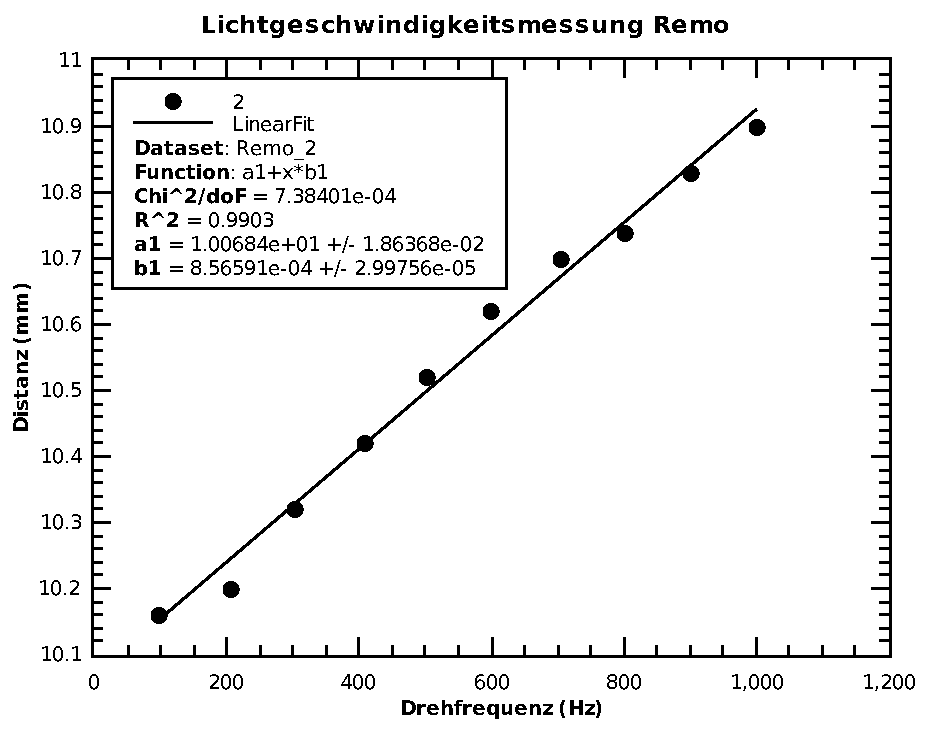
\includegraphics[width=.8\textwidth]{images/x-f-remo.pdf}
    \caption{Lineare Regression zur Berechnung des Faktors $b$, Messdaten von Remo Suter}
    \label{fig:x-f-remo}
\end{figure}

\begin{figure}[H]
    \center
    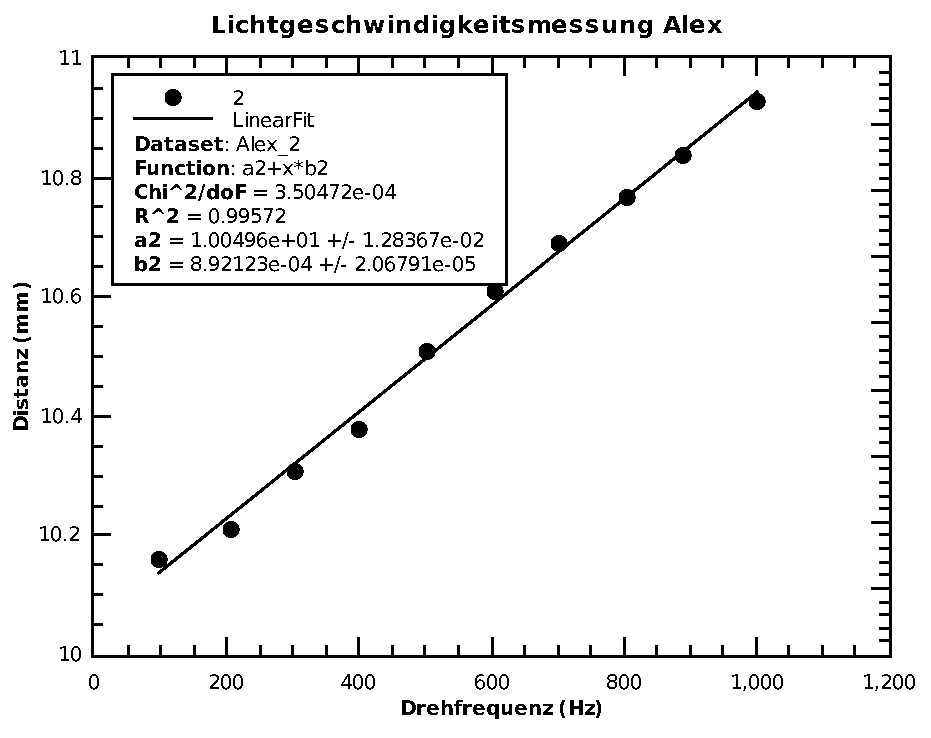
\includegraphics[width=.8\textwidth]{images/x-f-alex.pdf}
    \caption{Lineare Regression zur Berechnung des Faktors $b$, Messdaten von Alex Murray}
    \label{fig:x-f-alex}
\end{figure}

Die Punkte wurden nach der Formel \ref{eq:lichtgeschwindigkeit} gefittet und damit ergeben sich  die zwei  Faktoren:
\begin{align}
    b_{Remo} = \overline{b_{Remo}} \pm s_{\overline{b_{Remo}}} = (856.59 \pm 29.96)\cdot 10^{-6}
    b_{Alex} = \overline{b_{Alex}} \pm s_{\overline{b_{Alex}}} = (892.12 \pm 20.68)\cdot 10^{-6}
\end{align}


\subsection{Kalibrationsmessung}

In    den   Tabellen   \ref{tab:am-x-z}   und    \ref{tab:ym-x-z}    sind    die
Kalibrationsmessungen von Alex Murray  und  Yohannes  Measho aufgef\"uhrt. Beide
haben   die   gleiche   Messung   unabh\"angig  von   einander   durchgef\"uhrt.

\begin{figure}[H]
    \center
    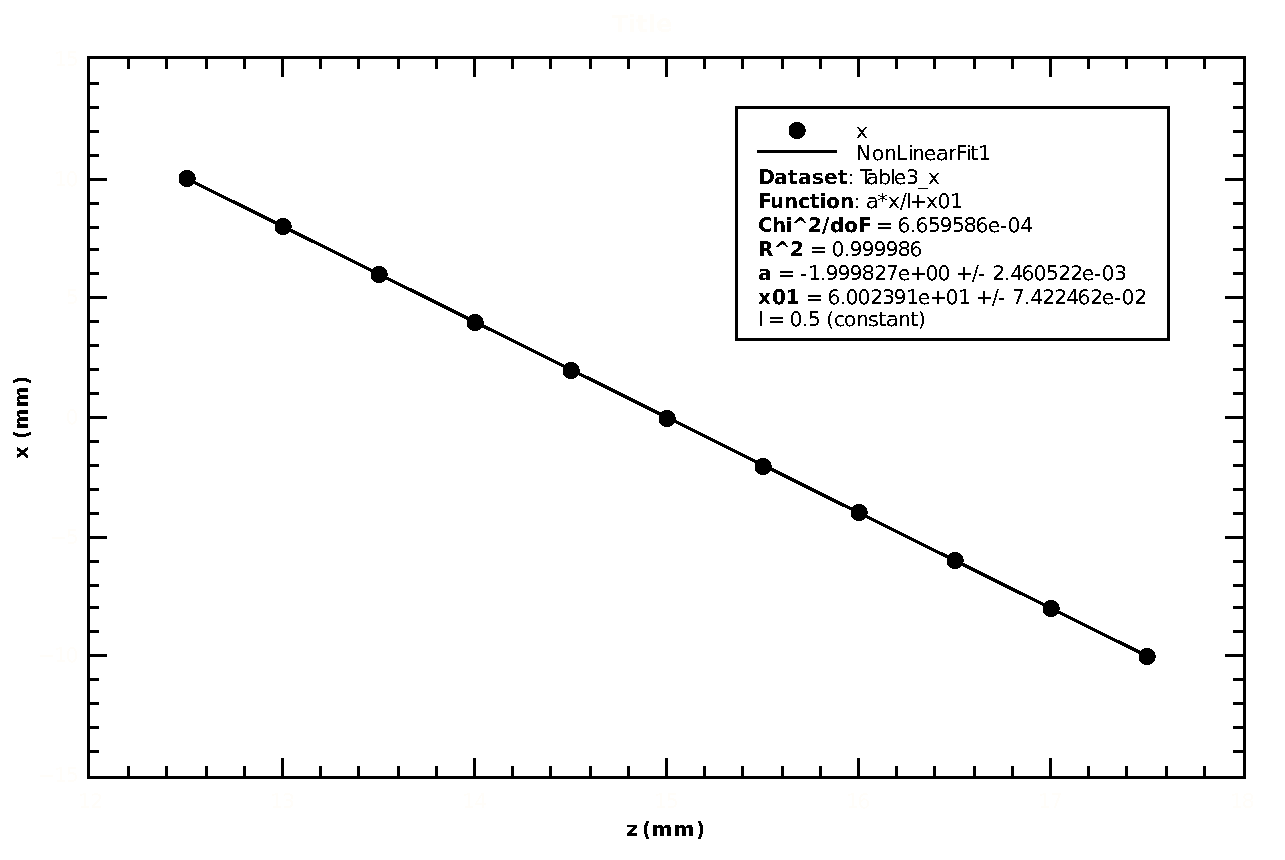
\includegraphics[width=.8\textwidth]{images/am-x-z-fit-a.pdf}
    \caption{Lineare Regression zur Berechnung des Faktors $a$ anhand der Kalibrationsmessung, Messdaten von Alex Murray}
    \label{fig:am-x-z-fit-a}
\end{figure}

In der Abbildung \ref{fig:am-x-z-fit-a}  sind  die  Messpunkte  von  der Tabelle
\ref{tab:am-x-z} als XY-Scatter Plot dargestellt.  Die  Punkte  wurden  nach der
Formel  \ref{eq:kalibration-a}   gefittet  und  somit  ergibt  sich  der  Faktor
$a_{Alex}$ als:
\begin{equation}
    a_{Alex} = \overline{a_{Alex}} \pm s_{\overline{a_{Alex}}} = -(1999.827 \pm 2.461)\cdot 10^{-3}
    \label{eq:am-a}
\end{equation}

\begin{figure}[H]
    \center
    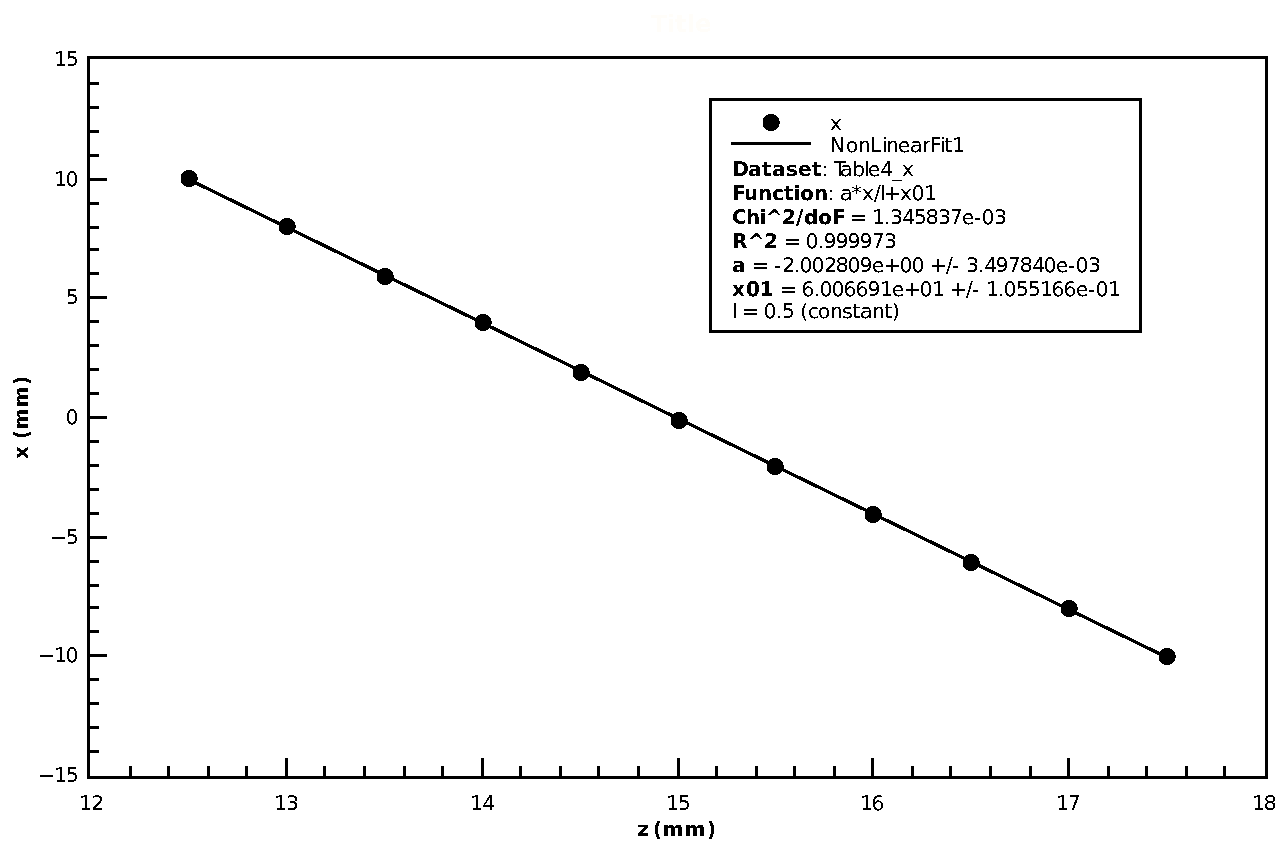
\includegraphics[width=.8\textwidth]{images/ym-x-z-fit-a.pdf}
    \caption{Lineare Regression zur Berechnung des Faktors $a$ anhand der Kalibrationsmessung, Messdaten von Yohannes Measho}
    \label{fig:ym-x-z-fit-a}
\end{figure}

In  der  Abbildung \ref{fig:ym-x-z-fit-a} sind die Messpunkte  von  der  Tabelle
\ref{tab:ym-x-z} als XY-Scatter Plot dargestellt. Die  Punkte  wurden  nach  der
Formel  \ref{eq:kalibration-a}   gefittet  und  somit  ergibt  sich  der  Faktor
$a_{Yohannes}$ als:
\begin{equation}
    a_{Yohannes} = \overline{a_{Yohannes}} \pm s_{\overline{a_{Yohannes}}} = -(2002.809 \pm 3.498)\cdot 10^{-3}
    \label{eq:ym-a}
\end{equation}
